\documentclass[danish]{report}
\usepackage[T1]{fontenc}
\usepackage[utf8]{inputenc}
\usepackage[danish]{babel}
\usepackage{listings}
\usepackage{color}
\usepackage{courier}
\usepackage{parskip}
\usepackage{graphicx}
\usepackage{amsfonts}
\usepackage{tabularx}
\usepackage{titlesec, blindtext, color}

\definecolor{dkgreen}{rgb}{0,0.6,0}
\definecolor{gray}{rgb}{0.5,0.5,0.5}
\definecolor{mauve}{rgb}{0.58,0,0.82}
\definecolor{gray75}{gray}{0.75}
\definecolor{light-gray}{gray}{0.5}
\newcommand{\hsp}{\hspace{20pt}}
\titleformat{\chapter}[hang]{\Huge\bfseries}{\thechapter\hsp\textcolor{gray75}{|}\hsp}{0pt}{\Huge\bfseries}
\titlespacing*{\chapter}{0cm}{-20pt}{10pt}
\setcounter{secnumdepth}{3}
\setcounter{tocdepth}{2}

\lstset{
  frame=,
  language=C,
  aboveskip=3mm,
  belowskip=3mm,
  showstringspaces=false,
  columns=flexible,
  basicstyle={\small\ttfamily},
  numbers=none,
  numberstyle=\tiny\color{gray},
  keywordstyle=\color{blue},
  commentstyle=\color{dkgreen},
  stringstyle=\color{mauve},
  breaklines=true,
  breakatwhitespace=true
  tabsize=4
}

% Title Page
\title{Obligatorisk opgave 3: Linux modules}
\author{Jacob B. Cholewa \& Mathias Pedersen }

\begin{document}
\maketitle
\begingroup
\let\clearpage\relax
\chapter{Introduktion}
I denne rapport arbejdes med tredje obligatoriske opgave i kurset Operativsystemer og C. Vi vil arbejde med koncepter som Macroer, linkedlists og moduler i linuxkernen.

\vspace{20 mm}\chapter{Metode}
I opgaven er stillet en række problemstillinger som skal løses på bedste vis. Alle opgaverne har fokus på C kode, som vi vil afvikle på en Ubuntu Linux virtuel boks. Opgaverne vil kræve implementering, og disse implementeringer vil blive forklare i længden af denne rapport. Vores løsninger testes under implementeringen på logisk basis og derefter ved observering af det afviklede programs opførsel.
\endgroup
\chapter{Teori}
\section{Linux kernen og moduler}

Et operativ system tilbyder et miljø til at køre programmer og tilbyder funktioner til at hjælpe bruger, som fx bruger grænseflade, program eksekvering, I/O tilgang, kommunikation mellem programmer og fejl håndtering. Operativ systemmet håndtere også andre opgaver som ressource allokering, sikkerhed og brugerstyring. De tre sidste nævnte er ikke så meget for at hjælpe brugeren, men for at sikre effektiv brug af resurser på systemmet.

Vi bruger til denne opgave operativ systemmet Linux. Linux bygger på UNIX kernen som er en lagdelt kerne (se figur \ref{fig:unix}). Linux kernen indeholder kun core funktioner tilbudt gennem en masse system kald til at bruge hardwaren i computeren, som fx system kaldet open som kan åbne en fil. Linux implementer en stor del af interfacet POSIX, Portable Operating System Interface, som er en standard der ensarter systemkald så kode kan benyttes på tværs af forskellige UNIX implementeringer (OSX, Solaris, mv.). Man har mulighed for at udvide Linux kernen med moduler. Fordelen ved at skrive kerne moduler er at man har direkte adgang til kernen og derfor kan bruge kernens systemkald og herunder POSIX interfacet direkte.

\begin{figure}
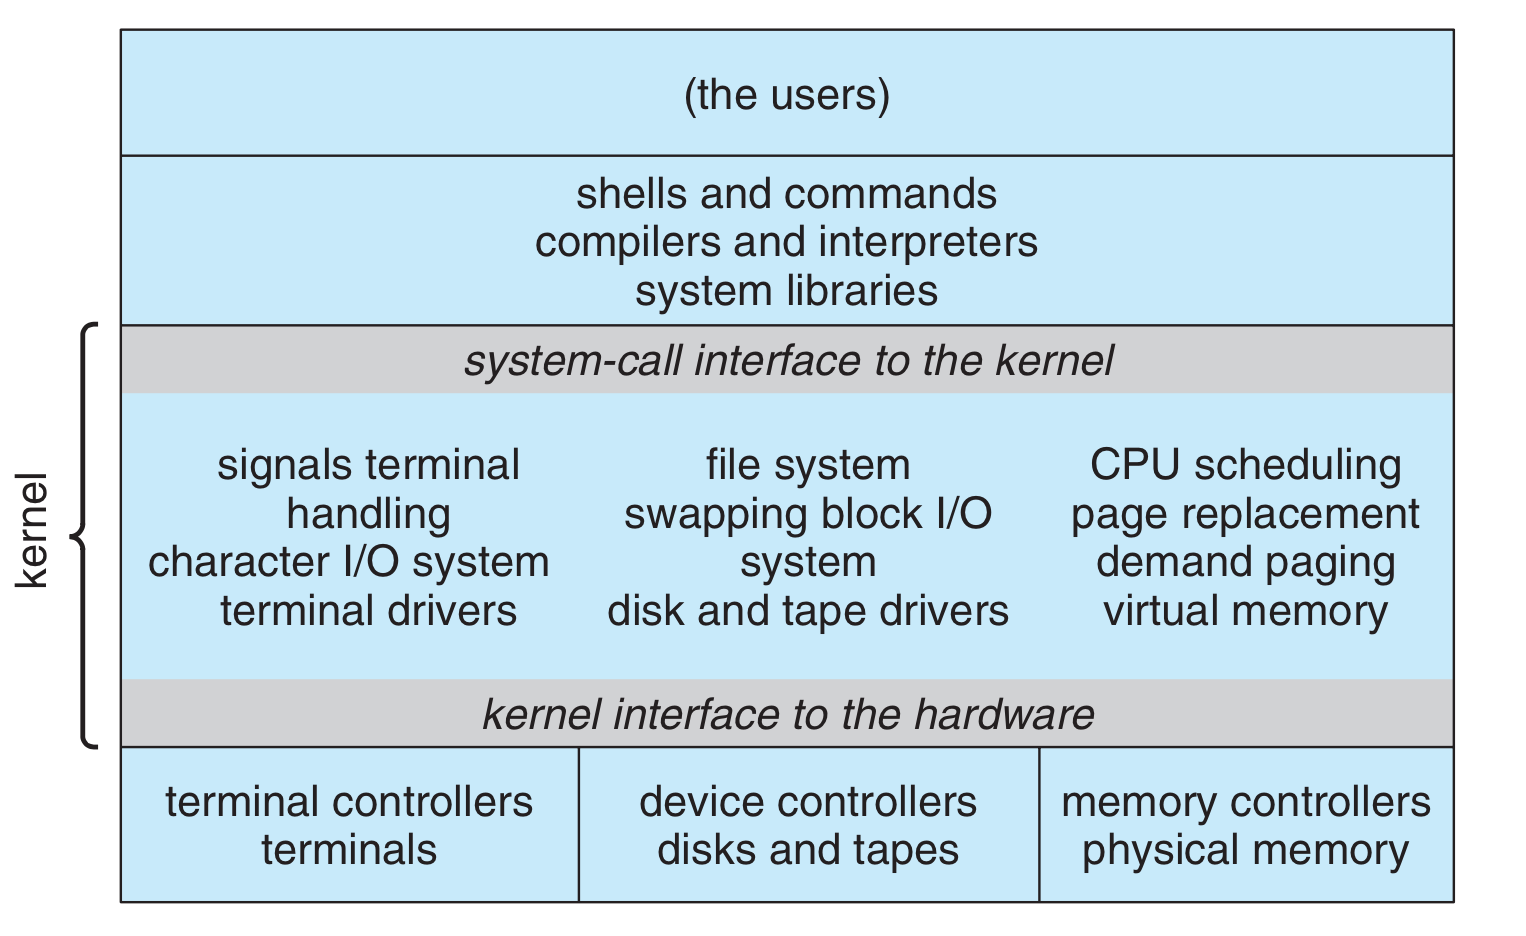
\includegraphics[width=\linewidth]{img/kernel.png}
\caption{Traditionel UNIX system struktur.}
\label{fig:unix}
\end{figure}

Linux kerne moduler er kodestykker som dynamisk kan loades og unloades en kørende linux kerne. De skal have en \textit{module\_init} og \textit{module\_exit} metode, som hhv. afvikles når modulet loades og unloades. Da moduler er del af kernen kan de bruge systemkald direkte.

\section{Macro metoder i C}

I C har man mulighed for at definere macro metoder. En macro er et stykke kode fragment som man knytter til et macro navn. Når navnet bruges i koden vil preprocessoren indsætte kode fragmentet. Nedenfor ses macroen \texttt{min} og hvordan preprocessoren indsætter kodefragmentet ved brug.
\begin{lstlisting}
#define min(X, Y)  ((X) < (Y) ? (X) : (Y))
x = min(a, b);          // x = ((a) < (b) ? (a) : (b));
y = min(1, 2);          //y = ((1) < (2) ? (1) : (2));
z = min(a + 28, *p);    //z = ((a + 28) < (*p) ? (a + 28) : (*p));
\end{lstlisting}

\section{Taskstruct og Linkedlist i Linuxkernen}

Biblioteket \texttt{<linux/list.h>} er en linkedlist implimentation i Linux. Implementationen bygger på structen \texttt{list\_head}. Structen indeholder en pointer til det næste og forrige element og på den måde kan man lave en liste af elementer.

\begin{lstlisting}
struct list_head {
    struct list_head *next, *prev;
};
\end{lstlisting}

Til at traversere listen kan man bruge list\_for\_each\_entry macroen

\begin{lstlisting}
/**
 * list_for_each_entry  -       iterate over list of given type
 * @pos:        the type * to use as a loop cursor.
 * @head:       the head for your list.
 * @member:     the name of the list_struct within the struct.
 */
#define list_for_each_entry(pos, head, member) \
    for (pos = list_entry((head)->next, typeof(*pos), member); \
        prefetch(pos->member.next), &pos->member != (head); \
            pos = list_entry(pos->member.next, typeof(*pos), member))
\end{lstlisting}

Macroen tager, givet det første element, og løber listen i gennem ved hele tiden af tage elementets next, altså det næste element, indtil enden af listen af nået.

En af de andre biblioteker der benytter linkedlist implementationen er \texttt{<linux/sched.h>}. En del af \texttt{sched} er \texttt{task\_struct}. Denne struct bruges til at holde information om processer der kører på systemmet. Structen indeholder også information om processens børneprocess. Derfor kan vi traversere gennem process træet og finde alle processer der køre på systemmet.

\begin{lstlisting}
struct task_struct {
    ... fields ...
    struct list_head children;      /* list of my children */
    struct list_head sibling;       /* linkage in my parent's children list */
}
\end{lstlisting}

For at kunne traversere processtræet har vi brug for den process som er forældre til alle andre processer i systemet. Denne process, init processen, er gemt i \texttt{init\_task} feltet i \texttt{<linux/sched.h>}

\section{Dybde først søgning}
DFS, eller Dybde først søgning, er en algoritme til at løbe en graf igennem. Algoritmen består af en stak. Hver gang man tager et element af stakken ligger man alle de ikke allerede besøgt elementer man kan nå fra elementet på stakken. Derefter forsættes processen indtil der ikke er flere elementer på stakken. På det tidspunkt vil man have besøgt alle elementer.

Da C er et stak sprog behøver man ikke et stak da program flowet naturligt vil følge en staks opførsel.


\chapter{Implementation}
\begingroup
\let\clearpage\relax
\section{Simple mod}

Dette eksempel (se fuld program kode i bilag \ref{simple.c}) er et linux modul som indeholder personers fødselsdag og printer fødselsdagene til \textit{kernel output}. Vi har altså derfor brug for en struct til at holde information om personer fødselsdag.

\begin{lstlisting}
typedef struct birthday {
        int day;
        int month;
        int year;
        struct list_head list;
} Birthday;
\end{lstlisting}

I vores module init metode opretter vi en liste personer. Vi bruger kmalloc til at allokere hukommelse til structen og fylder den derefter med personens data. kmalloc() er ligesom malloc() som allokerer hukommelse, men virker i kernel moduler. Derefter itererer vi ved hjælp af \texttt{list\_for\_each\_entry} igennem den liste vi lige har oprettet og printer alle personernes fødselsdag til \textit{kernel output}.

Når modulet bliver fjernet igen kaldes modulets exit metode hvor vi igen itererer over listen for at fjerne personerne og deallokerer hukommelsen igen. Her bruger vi en speciel iterator macro som ikke fejler hvis man fjerner elementer under itereringen.

\section{Tasklist mod}
I denne opgave skal vi meget som den forrige iterere over en linked list og udskrive information. I denne opgave drejer det sig om kørende processor på systemet. Opgaven lyder på at løbe gennem processorne med en dybde først søgning og udskrive visse informationer om dem. Al udprintning sker til \textit{kernel output} med \textit{printk()} funktionen.

For at kunne lave en dybde først søgning har vi oprettet en metode som vil bruges rekursivt. Metoden hedder \textit{dfs} og koden ses herunder.

\begin{lstlisting}
void dfs(struct task_struct *tsk, struct list_head *ptr){
	//Struct used for holding current task
	struct task_struct *task;
	
	//For each children of the tsk task
	list_for_each(ptr, &tsk->children){ 
	
		//Gets a pointer to the next element
		task = list_entry(ptr, struct task_struct, sibling); 
		
		//Prints information about the task
		printk(KERN_INFO "%d %s\n", task->pid, task->comm);
		
		//Call resurcivly on the current task
		dfs(task,list);
	}
}
\end{lstlisting}

Metoden tager to parametre.

\begin{itemize}
	\item \textbf{*tsk} er en pointer til et task element
	\item \textbf{*ptr} er en pointer til hvor vi er i dette hirakis liste over søskende
\end{itemize}

\textit{list\_for\_each} fungerer som vores while condition der sikre at vi ikke løber over listens lændge. \textit{list\_entry} bruges til at få en pointer til det næste element i dette hiraki. Da det nu er en pointer til et barn vi har, beder vi om en pointer til den næste søskende i hirakiet.

På den måde får vi udskrevet strukturen i dybden først, da vi altid tager grenene til bunds før vi går til søskende elementer.

\vspace{20 mm}\chapter{Konklusion}
I denne opgave har vi løst stillede opgaver med implementering og derefter verificeret at koden virker.
\endgroup
\appendix
\chapter{Simple module}
\label{simple.c}

\section{Simple.c}
\begin{lstlisting}
#include <linux/init.h>
#include <linux/module.h>
#include <linux/kernel.h>
#include <linux/list.h>
#include <linux/types.h>
#include <linux/printk.h>
#include <linux/slab.h>


typedef struct birthday {
    int day;
    int month;
    int year;
    struct list_head list;
} Birthday;

//struct list_head birthday_list;
static LIST_HEAD(birthday_list);

/* This function is called when the module is loaded. */
int simple_init(void)
{
        printk(KERN_INFO "Loading Module\n");
        
        int i;
        
        for (i = 1; i <= 5; i++){
            Birthday *person;
            person = kmalloc(sizeof(*person), GFP_KERNEL);
            person->day = i;
            person->month= 8;
            person->year = 1995;
            INIT_LIST_HEAD(&person->list);
            list_add_tail(&person->list, &birthday_list);
            printk(KERN_INFO "added\n");
        }
        
        // for each loop over linked list
        Birthday *p;
        list_for_each_entry(p, &birthday_list, list) {
            printk(KERN_INFO "%d-%d-%d\n", p->day, p->month, p->year);
        }
        
       
        return 0;
}

/* This function is called when the module is removed. */
void simple_exit(void) {
    printk(KERN_INFO "Removing Module\n");
    
    Birthday *ptr, *next;
    list_for_each_entry_safe(ptr,next,&birthday_list,list) {
        /* on each iteration ptr points */
        /* to the next birthday struct */
        list_del(&ptr->list);
        printk(KERN_INFO "removed elm %d\n", ptr->day);
        kfree(ptr);
    }
}

/* Macros for registering module entry and exit points. */
module_init( simple_init );
module_exit( simple_exit );

MODULE_LICENSE("GPL");
MODULE_DESCRIPTION("Simple Module");
MODULE_AUTHOR("SGG");


\end{lstlisting}

\section{Makefile}
\begin{lstlisting}
obj-m += simple.o
all:
    make -C /lib/modules/$(shell uname -r)/build M=$(PWD) modules
    sudo rmmod simple
    sudo insmod simple.ko
clean:
    make -C /lib/modules/$(shell uname -r)/build M=$(PWD) clean

\end{lstlisting}

\chapter{Tasklist module}
\label{tasklist.c}

\section{tasklist.c}
\begin{lstlisting}
#include <linux/init.h>
#include <linux/module.h>
#include <linux/kernel.h>
#include <linux/list.h>
#include <linux/printk.h>
#include <linux/sched.h>

void dfs(struct task_struct *tsk, struct list_head *ptr){
    //Struct used for holding current task
    struct task_struct *task;

    //For each children of the tsk task
    list_for_each(ptr, &tsk->children){ 
            
        //Gets a pointer to the next element
        task = list_entry(ptr, struct task_struct, sibling); 

        //Prints information about the task
        printk(KERN_INFO "%d %s\n", task->pid, task->comm);

        //Call resurcivly on the current task
        dfs(task,ptr);
    }
}

/* This function is called when the module is loaded. */
int tasklist_init(void)
{
    //Printing to the kernel info output that we're loading the module
    printk(KERN_INFO "Loading Module\n");

    //Defining a list_head struct to use as a loop cursor
    struct list_head *ptr;

    //Call the DFS algorithm on the init_task (The mother of all tasks)
    dfs(&init_task, ptr);       

    return 0;
}


/* This function is called when the module is removed. */
void tasklist_exit(void) {
    printk(KERN_INFO "Removing Module\n");
    
}

/* Macros for registering module entry and exit points. */
module_init( tasklist_init );
module_exit( tasklist_exit );

MODULE_LICENSE("GPL");
MODULE_DESCRIPTION("Tasklist Module");
MODULE_AUTHOR("SGG");
\end{lstlisting}

\section{Makefile}
\begin{lstlisting}
obj-m += tasklist.o
all:
    make -C /lib/modules/$(shell uname -r)/build M=$(PWD) modules
remove: 
    sudo rmmod tasklist
install:
    sudo insmod tasklist.ko
reinstall:
    sudo rmmod tasklist
    sudo insmod tasklist.ko
clean:
    make -C /lib/modules/$(shell uname -r)/build M=$(PWD) clean
\end{lstlisting}

\end{document}          
